\chapter{Introduction}
\chapterauthor{D. Be{\ss}ler, S. Koralewski, M. Pomarlan}

This document, referred to as the ``\neem Handbook'' hereafter,
describes the \ease system for episodic memories of everyday activities.
%The \neem Handbook will be updated along the progress in the CRC \ease.
It is thought to provide \ease researchers with compact but still comprehensive
information about what information is contained in \neems,
how it is represented, acquired, curated and published.

\begin{figure}[h!]
\centering
\begin{tikzpicture}[
    border/.style={draw=easeblue},
    dark/.style={border,fill=easeblue!20},
    light/.style={border,fill=easeblue!10},
    lighter/.style={border,fill=easeblue!5},
    heading/.style={text=easeblue,font=\bf,text badly centered},
    label1/.style={text=easeblue,text badly centered},
    label2/.style={text=black,text badly centered,font=\it},
    label/.style={text=black,text width=1.7cm,text badly centered},
    hexagon/.style={regular polygon,regular polygon sides=6,rounded corners},
    triangle/.style={regular polygon,regular polygon sides=3,rounded corners},
    trapez/.style={font=\bf,text badly centered,trapezium,trapezium angle=60,rounded corners},
    user/.style={hexagon,lighter,minimum width=2.5cm,inner sep=0},
    img/.style={}
]
  %\draw[help lines](-4,-4)grid(4,3);
  %% outer hexagon
  \node[hexagon,dark,minimum width=5.0cm] (OUTER) {};
  \node[heading] at (0,-1.8) (ACQ) {acquisition};
  \node[heading,rotate around={120:(OUTER)},rotate=180] at (ACQ) {curation};
  \node[heading,rotate around={-120:(OUTER)},rotate=180] at (ACQ) {publication};
  %% inner triangle
  \node[triangle,light,minimum width=6.0cm] at (OUTER) (INNER) {};
  %% inner trapez
  \node[trapez,lighter,
    minimum height=21mm,yshift=-0.275cm] at (INNER.center) (LIB) {};
  \node[label,yshift=0.2cm] at (INNER) (BG) {NEEM Background};
  \node[label,below=0.2cm of BG.south,anchor=north east] (NAR) {NEEM Narrative};
  \node[label,below=0.2cm of BG.south,anchor=north west] (EXP) {NEEM Experience};
  \draw[draw=easeblue] (BG.south west) -- (BG.south east);
  \draw[draw=easeblue] (NAR.north east) -- (NAR.south east);
  %% heading
  \node[label1,text width=14mm,above=0.4cm of BG] (HUB1) {NEEM HUB};
  %%
  \node[user,text=black,anchor=north,yshift=-0.2cm,
    path picture={\node[yshift=1.8cm] at (path picture bounding box.center){
        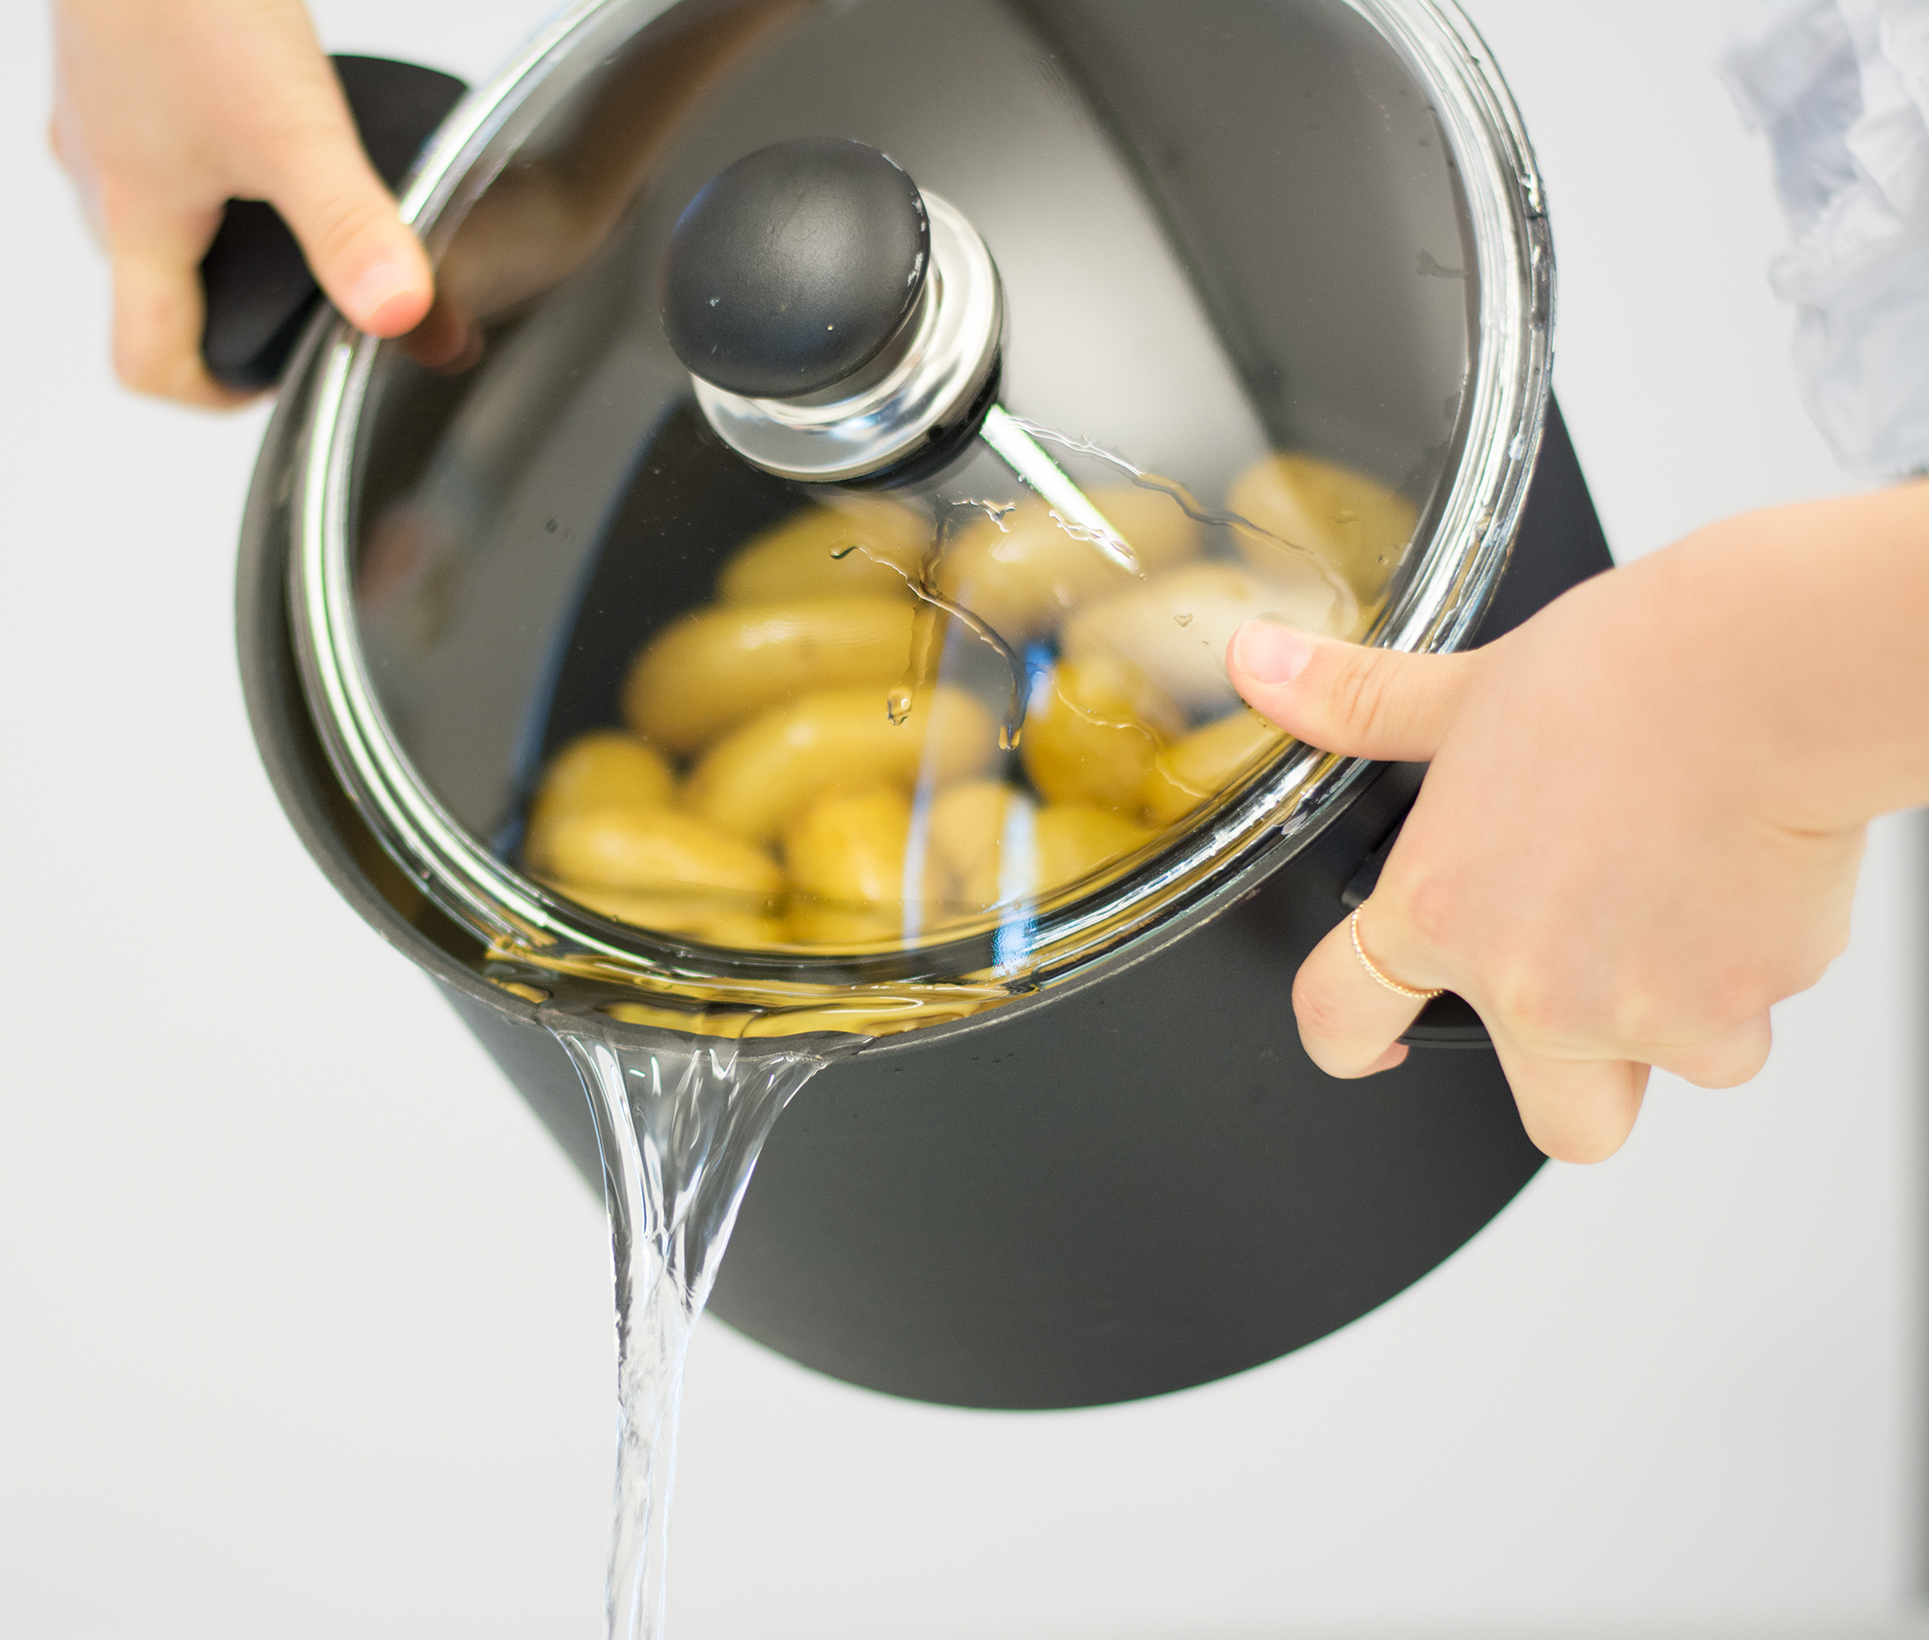
\includegraphics[width=2.55cm]{img/topf-2.jpg}
    };}
  ] at (OUTER.south) (X1) {};
  \node[user,anchor=center,yshift=-0.4cm,xshift=2.4cm,
    path picture={\node[yshift=0.0cm] at (path picture bounding box.center){
        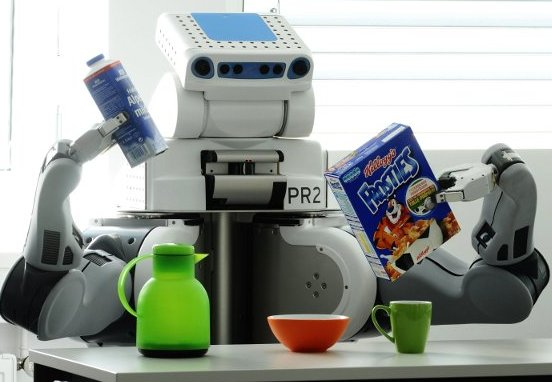
\includegraphics[height=2.55cm]{img/pr2_milk_frosties_small_top.jpg}
    };}
  ] at (X1.north) (X2) {};
  \node[user,anchor=center,yshift=-0.4cm,xshift=-2.4cm,
    path picture={\node[yshift=0.0cm] at (path picture bounding box.center){
        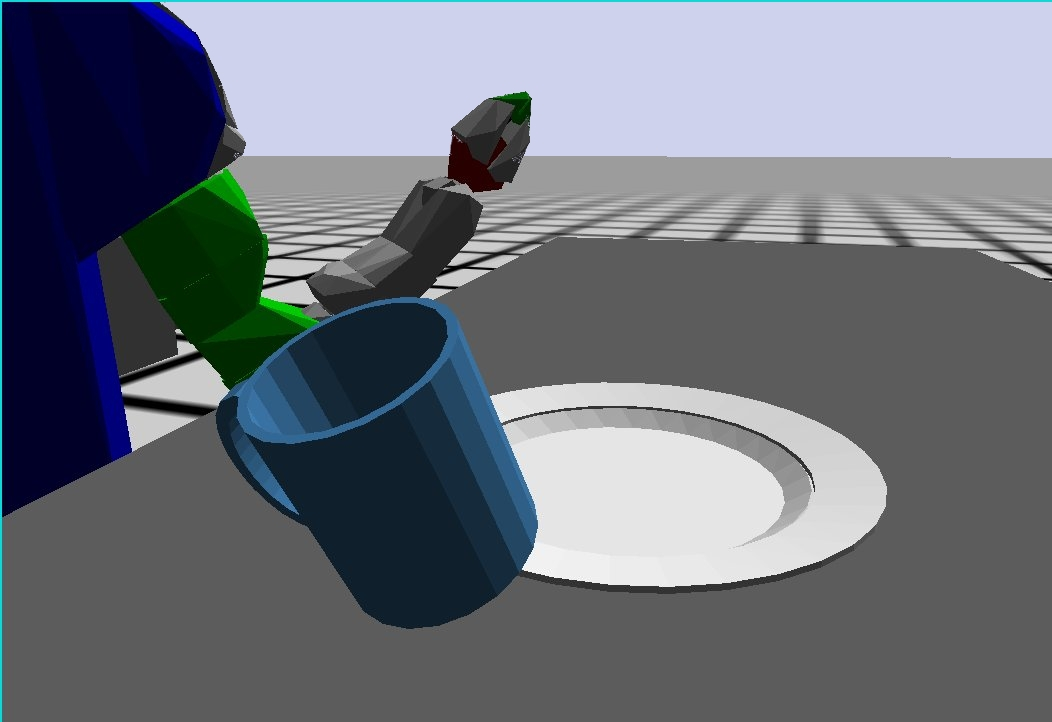
\includegraphics[height=2.55cm]{img/cup-on-plate-unstable-final.jpg}
    };}
  ] at (X1.north) (X5) {};
  \node[user,rotate around={120:(OUTER)},
    path picture={\node[yshift=0.0cm] at (path picture bounding box.center){
        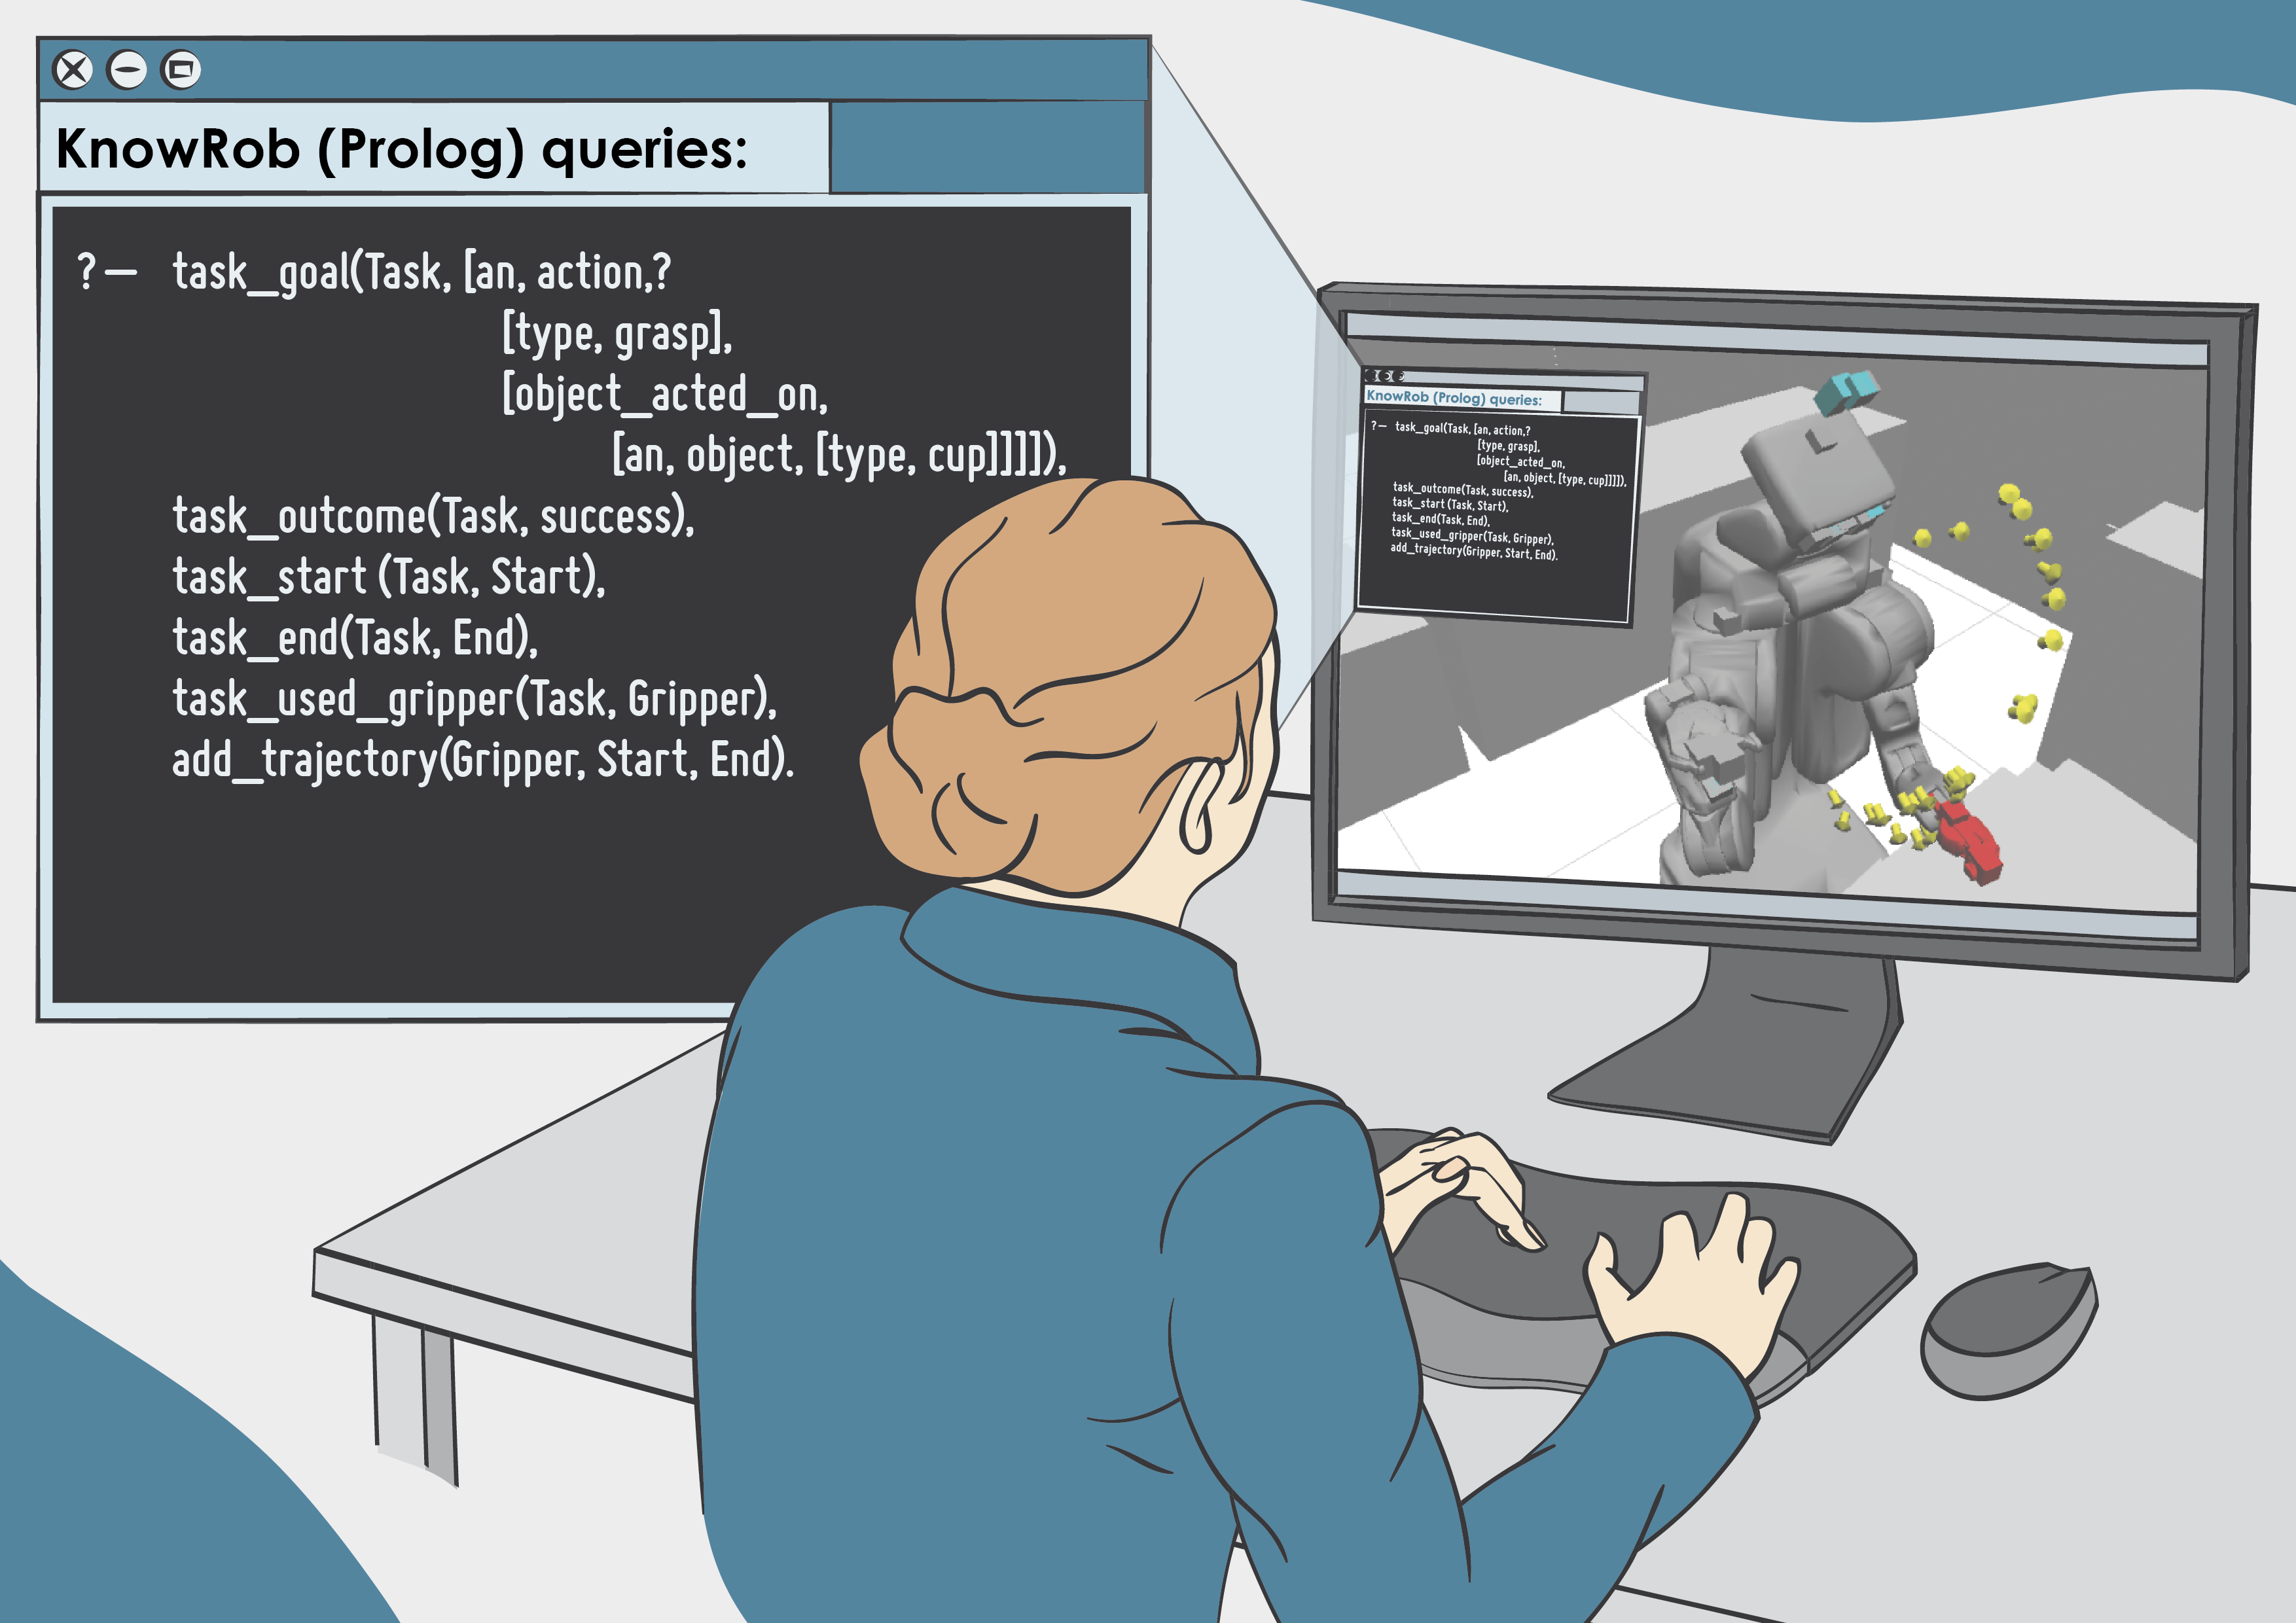
\includegraphics[height=2.55cm]{img/Programmer.png}
    };}
  ] at (X1) (X3) {};
  \node[user,rotate around={-120:(OUTER)},
    path picture={\node[yshift=0.0cm] at (path picture bounding box.center){
        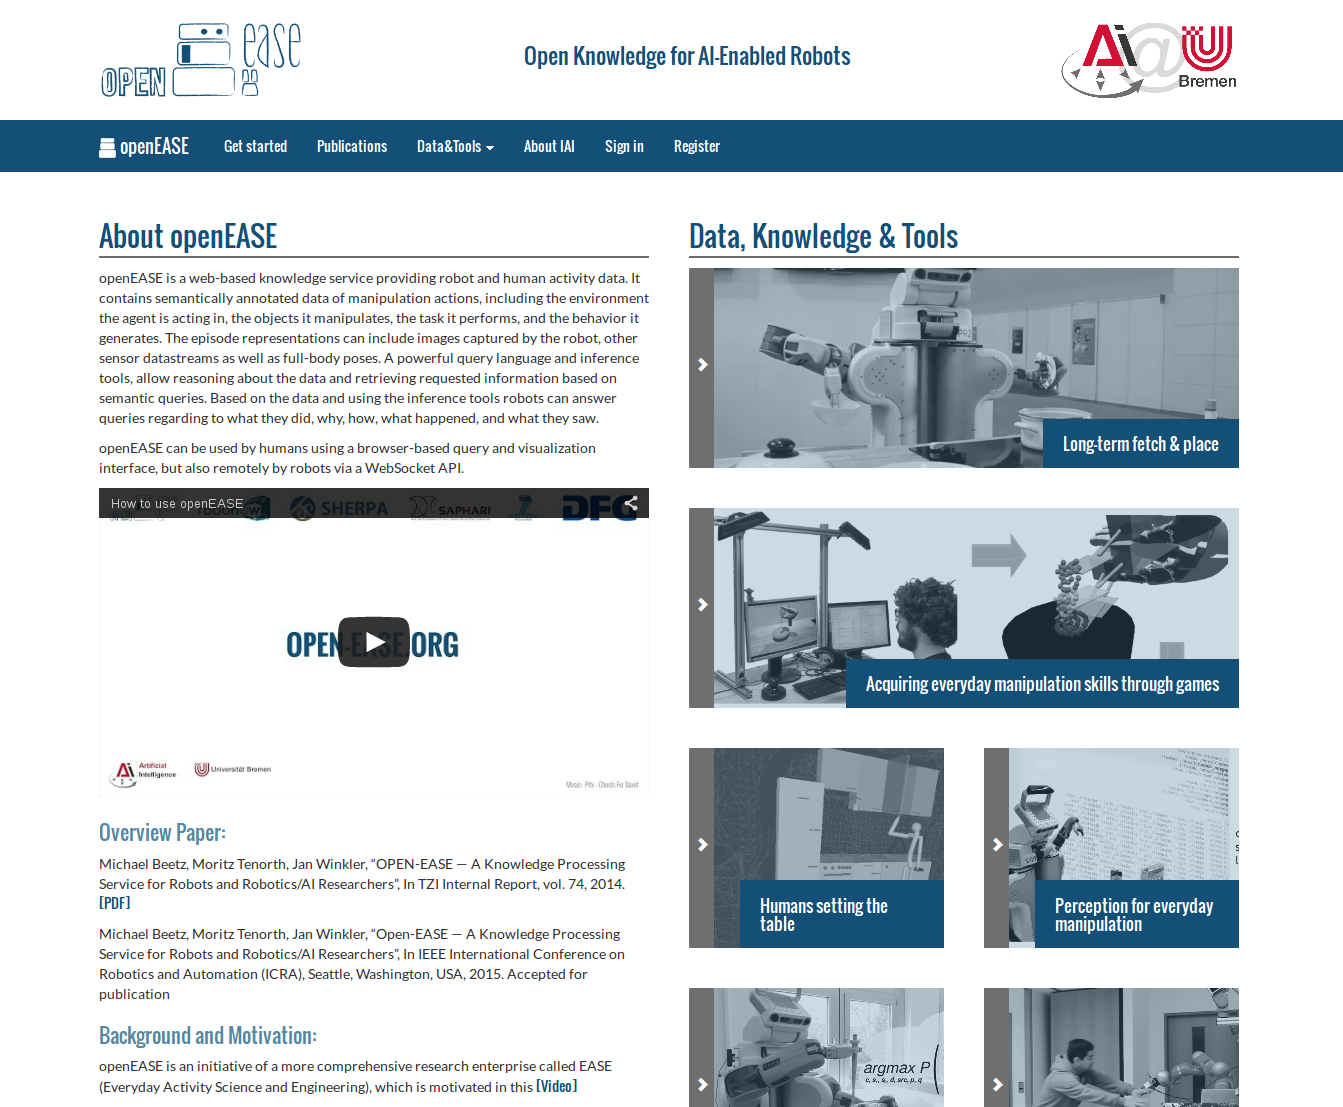
\includegraphics[height=2.55cm]{img/open-ease-web-page-full_cropped.png}
    };}
  ] at (X1) (X4) {};
  %%
  \node[label2,anchor=north] at (X1.south) {observation};
  \node[label2,anchor=north] at (X2.south) {experimentation};
  \node[label2,anchor=north] at (X5.south) {simulation};
  
\end{tikzpicture}
\caption{The EASE system for acquisition, curation and publication of episodic memories}
\label{fig:architecture}
\end{figure}

\paragraph{Narrative Enabled Episodic Memories}
% From KnowRob 2.0
When somebody talks about the deciding goal in the last soccer world championship many of us can ``replay'' the episode in our ``mind's eye''.
Those episodic memories can be seen as abstract descriptions that allow us to recall detailed pieces of information from any experienced activity.
Having those detailed memories, we can use them to learn general knowledge or map similar memories to unknown situations, so we know how to behave in the given situation.
\todo{DB: refer to Figure~\ref{fig:architecture}}

% From KnowRob 2.0
\ease integrates episodic memories deeply into the knowledge acquisition, representation, and processing system. 
For every activity the agent performs, observes, prospects and reads about, it creates an episode and stores it in its memory.
An episode is best understood as a video recording that the agent makes of the ongoing activity.
In addition, those videos are enriched with a very detailed story about the actions, motions, their purposes, effects and the agent's sensor information during the activity.

% From KnowRob 2.0
We define the episodic memories created by our system narrative-enabled episodic memories (\neems).
A \neem consists of the \emph{\neem experience} and the \emph{\neem narrative}.
The \neem experience captures low-level data such as the agent's sensor information, e.g. images and forces, and records of poses of the agent and its detected objects.
\neem experiences are linked to \neem narratives, which are stories of the episode described symbolically.
These narratives contain information regarding the tasks, the context, intended goals, observed effects, etc.
The \neemexp and \neemnar combined are so rich of information that the agent can replay an episode to experience the seen activity anytime again.

\neems are representations of experiences acquired through experimentation, reading, observing, mental simulation, etc.
The main goal is to establish a common vocabulary used to annotate experience data across different tasks, scientific disciplines, and modalities of acquisition, and to define models for the representation of experience data.
The vocabulary is not just a set of atomic labels, but each label has a formal definition in an ontology.
These definitions are done such that a set of \emph{competency questions} about an activitiy can be answered by a knowledge base that is equipped with the ontology and a collection of \neems.

The \neem model is formally defined in form of an \owl ontology which is based on the DOLCE+DnS Ultralite (DUL) upper-level ontology~\cite{DOLCE2003}.
DUL is a carefully designed ontology that seeks to model general categories underlying human cognition without making any discipline-specific assumptions.
Our extensions of DUL mainly focus on characterizing different aspects of activities that were not considered in much detail in DUL, but are relevant for the autonomous robotics scope.
These extensions are part of an ontology that we have called
\soma~\footnote{\url{https://ease-crc.github.io/soma}}.
A \neem is made of several patterns defined either in \dul or in \soma.

While it is possible to create the representations listed in this document through a custom exporter, it is not advised to do so.
Instead, it is advised to interface with the
\knowrob knowledge base~\footnote{\url{https://github.com/knowrob/knowrob}}.
\knowrob provides an interface based on predicate logics that allows to interact with \neems.
The language is a collection of predicates that can be called by users to ask certain types of competency questions covering different aspects of activitiy, or to add labels and relationships in the \neemnar.
We will provide example expressions in this document that highlight how the knowledge base can be used to interact with \neems.

% paragraph about generalizability of robot behaviour (add reference to Pratt paper ``Is a Cambrian Explosion Coming for Robotics?'')
\lipsum[4]
\todo{DB: write paragraph about generalizability, Pratt paper ``Is a Cambrian Explosion Coming for Robotics?''}

% % % % % % % % % % % % % % % % %
% % % % % % % % % % % % % % % % %
\section{Notation} % Domain of Discourse
\label{sec:notation}

In this Section, we will shortly introduce the notions and notations that are important to follow this document.
%Because in subsequent sections we will give more formal definitions for various concepts, we now review some basic notions about the main formalism we use in the ontology, as well as introduce the notation we will employ.

%%% ABOX -- TBOX
\neems are formally represented using an \emph{ontology}.
An ontology is a collection of logical axioms in some formal language such as description logic (DL).
%In the case of many ontologies available in the semantic web, as well as in the case of SOMA, this formal language is description logic, also known as DL.
The entities that can be described in DL can be either \emph{concepts} (sometimes known as \emph{classes}),
and \todo{Seba: Can we here remove individuals?
It seems not very well definied that concepts are known as individuals and in the next sentence the instances are called individuals.} \emph{individuals}.
An individual is an instance of one or more concepts.
A concept may be subsumed by another.
Between individuals there may be relations called \emph{object properties},
and, in addition, an individual can also have \emph{data properties} that link it to some data values.
%As a syntactic convenience, an individual can also have ``data properties'' that link it to some alphanumeric data item which is itself not considered an individual in the ontology.
As an example, let us assume that Alice and Bob are both individuals of the concept \concept{Human},
and that the object property \relation{hasChild} connects Alice to Bob,
i.e. the relation asserts that Bob is a child of Alice.
We may also know the height of Alice, which would be represented by a data property \relation{hasHeight} whose value could be a string such as \emph{1,7m} to represent that she is 1.7m tall.
%%
In the following, to make clear when we are talking about concepts and when about individuals, we will denote the set of all concepts as $\mathcal{T}$ (called the TBox), and the set of all individuals as $\mathcal{A}$ (called the ABox).
%Accordingly, there are axioms that describe concepts or object/data properties,
%and axioms that describe individuals and the relations between them.
%The set of concepts, object and data properties, and the axioms that
%define them is called the Tbox, or terminological part,
%and we will denote it by $\mathcal{T}$.
%The set of individuals and the axioms describing them is called the Abox,
%or assertion part, and we will denote it by $\mathcal{A}$.

%%% formatting
It is useful when describing concepts to emphasize the concept names such that it is clear we reference the concept, and not the colloquial word. As such, \concept{Concepts} and \relation{relations} will be written in a different font.
Note that the name of a concept always starts with an uppercase letter, whereas the name of a relation with a lowercase one.
Any word appearing in a concept or relation name after the first one will always begin with an uppercase letter.

%%% namespaces
Ontologies are meant to build on one another, and it is not uncommon for an ontology to collect thousands of concepts from external ontologies it imports.
To prevent name clashes, in actual usage the names of concepts, relations, and individuals are often name-spaced.
In this document, since we mostly talk about concepts from the SOMA ontologies,
the namespace will not be made explicit.
An exception will be made in some diagrams where we reference concepts defined in more basic ontologies,
such as those used to define the Ontology Web Language (OWL).
An example is a name such as \emph{xsd:double}; in this case, \emph{xsd} is the namespace.

% % % % % % % % % % % % % % % % %
% % % % % % % % % % % % % % % % %
\section{Scope} % Domain of Discourse
\label{sec:scope}
%\todo{Mihai: write about competency questions here. Probably would be good to provide a list of them that we intend to cover with the information contained in neems}

Our work aims to provide knowledge modeling for robotic manipulation and autonomous robot control, such that data acquired through performing actions can be stored, interpreted, and used towards training and improving robot skills. \todo{DB: this leaves out the neem-hub/acquistion/data aspects}
The knowledge that is to be extracted from data must include aspects of interaction forces and motion characteristics of objects participating in an action, since it is these physical and geometric considerations that are crucial to determining whether, or to what degree, an action is successful. Collections of recorded episodes -- NEEMs -- will be used as training data for machine learned models. Further, the rich semantic annotations that accompany the data, and together with it form a ``narratively enabled episode memory'', enable querying and filtering the data, such that a robot can formalize a learning problem for itself and curate its training data to be appropriate for it. Information about how the data is collected, with what methods, from what agents, in which contexts, is important for this process, as machine learning techniques are sensitive to training data biases. Note that in principle episodes can be stored of any agent performing any activity, and in actuality many of the NEEMs we expect to store will come from humans demonstrating how to perform a task. NEEMs are therefore not simply intended as a kind of self-practice journal, but rather as a store of practical knowledge of a variety of agents, useful for a variety of autonomous, humanoid robots.

%Ideally, the knowledge we formalize in this collection of ontologies will allow a single, general control program to adapt itself, via reasoning, and generate adequate behavior in a large variety of settings, for different tasks and participating objects.
\todo{DB: I think this paragraph is focussed too much on the knowledge aspect. We should mention machine learning models that are to be trained from neems, collections of neems stored on the neem hub etc. }
% NOTE: taken from SOMA paper
%The broad scope of our work is everyday object manipulation tasks in autonomous robot control, and in particular the motion and force characteristics of objects that interact with each other.
%The research question driving us is whether a single general control program can be written that can generate adequate behavior in many different contexts: for different tasks, objects, and environments.
%\todo{somebody needs to rephrase this! it is copied from SOMA paper}

The kinds of knowledge a robot needs for competent performance of its tasks are varied. Usually, knowledge modelling in robotics and AI has focused on a symbolic level, of actions treated as black boxes that relate to a larger plan by means of their preconditions and effects. Actions are also very underspecified when described in spoken commands. This abstract level of description however is insufficient; the physical details of the actions matter. For example, the angle and speed with which a pitcher is moved, and the amount of liquid in it, determines whether there will be spillage. A robot needs to choose appropriate parameters for its actions, and infer these parameters when they are left unspecified in a command.
% NOTE: taken from SOMA paper
%One of the challenges is that, using such a general plan, the agent needs to fill the knowledge gaps between abstract instructions included in the plan and the realization of context specific behavior. That is, for example, the many ways of how humans perform a pouring task depending on the source from which is poured, the destination, and the substance that is to be poured.
%Another challenge is that object manipulation tasks may fail if the agent does not perform the motions competently and well. This is caused by the agent choosing inappropriate parametrization of its control-level functions.
%\todo{somebody needs to rephrase this! it is copied from SOMA paper}

Such inference requires the robotic agent to be equipped with common-sense and intuitive physics knowledge, as well as an abstract task and object model, and knowledge of how to apply these models in a given situation. SOMA is an attempt to support each of these requirements. A brief list of some of the over-arching competency questions follows.

%%\begin{itemize}
%%    \item \emph{How are actions conceptualized?} What is an Action, how does it relate to other concepts an Agent might have about the world? What is the purpose of an Action?
%%    \item \emph{How are possibilities for action formalized?} How does an agent model what is made available by the environment? How does an agent model what it is itself capable of?
%%    \item \emph{What is the structure of an Action?} How do several actions make up another? What objects participate in an action and with what roles?
%%    \item \emph{How are qualitative and quantitative features of the world represented?} What is the parameter set of an action? What regions can values for these parameters occupy? What is a good parameterization and how can one be found?
%%\end{itemize}

\begin{itemize}
    \item \emph{How are actions conceptualized?} What is an action, how does it relate to other concepts an agent might have about the world? What is the purpose of an action?
    \item \emph{What is the structure of an action?} How do several actions make up another? What objects participate in an action and with what roles?
    \item \emph{How are qualitative and quantitative features of the world represented?} What is the parameter set of an action? What regions can values for these parameters occupy? What is a good parameterization and how can one be found?
    \item \emph{How are the physical interactions that underlie an action described?} What are the involved forces, and how are they parameterized? What are relevant qualitative, and thus more general, descriptors for interactions, such as balance, blockage, compulsion? How are qualitative aspects of interaction grounded in quantitative physical phenomena?
    \item \emph{How are objects conceptualized?} What roles can an object play? What actions can it take part in? What kinds of objects are necessary for an action?
    \item \emph{How is an action recorded and described?} What is the relevant data to capture how an action unfolded? What are the relevant pieces of contextual information for describing an action that has actually occurred? What was the outcome of the action, in particular, to what extent did it match the goal?
    \item \emph{How is a learning problem formalized?} What is the optimization goal? What assumptions were in effect when collecting the training data? What sort of influence might biases have upon the learned model? What should be essential features that a learned model should use? What would be sanity checks on the learned model to verify it does not abuse spurious correlations?
\end{itemize}
\todo{DB: could we add some motion/force questions here?}
\todo{DB: could we add some questions that require a ML model learned from neems?}

% NOTE: taken from SOMA paper
%The employment of a general plan thus requires an abstract task and object model, and a mechanism to apply this abstract knowledge in situational context.
%To achieve this, an agent needs to be equipped with the necessary common-sense and intuitive physics knowledge, which is what SOMA\todo{The acronym is no where defined} attempts.
%\todo{somebody needs to rephrase this! it is copied from SOMA paper}

% % % % % % % % % % % % % % % % %
% % % % % % % % % % % % % % % % %
\section{Overview}
\label{sec:overview}

% paragraph about the intention behind this document
\neems are the central data structures that link research results of various sub-areas within the collaborative research center \ease.
\ease is an interdisciplinary institution headed by leading researchers in the fields robotics, human cognition, formal logics, and linguistics.\todo{is this complete?}
The overall goal is to make a robot more competent in performing everyday activities.
This is accomplished by equipping the robot with models learned over experiences represented as \neems.
The purpose of this document is to provide detailed information about the \ease system for episodic memories.
That is how \neems are
represented as knowledge bases linked to time-series data,
acquired through experimentation, observation or simulation,
stored on a centralized server, and
maintained as a dataset for the research community.
The architecture is shown in Figure~\ref{fig:architecture}, and will be summarized in the remainder of this section.

% paragraph about representation (neem background, narrative, experience)
At the core of the \ease system for episodic memories is the \neem data structure.
It is a heterogenous datastructure that contains data in different formats to represent different categories of information about everyday activities.
Each \neem is made of three parts: background (Chapter~\ref{ch:background}), narrative (Chapter~\ref{ch:narrative}) and experience (Chapter~\ref{ch:experience}).
The background represents physical activity context by characterizing the environment, and agents that play a role during the activity.
A single background may be shared in mutiple \neems.
The narrative is a representation of events that happened, their characterization and contextualization.
That is, for example, that an event occurred, what roles objects played during the event, how the event was carried out through motions and interactions, and what the reason of its occurrence is.
The narrative provides labels used to annotate the time-series data stored in the experience of the \neem.
This is done by associating the event time intervals to slices in the time-series database.
The experience data is used to capture some aspects of kinematics and dynamics of an activity, that is how objects moved, how they got into contact with each other, and how forces act upon objects.

% paragraph about neem hub -- purpose, potential, ... -- add some buzzwords from data science
\neems are stored on a publicly accessible infrastructure that we have called the \neemhub (Chapter~\ref{ch:neemhub}).
The \neemhub builds on top of common infrastructure used in data science to continuously update models learned from \neems.
Uploading a \neem requires to create a new data set on the \neemhub GitLab interface where users can provide documentation, usage examples, additional links and references for their \neem data set.
Once a user is satisfied with the state of the data set, it may be published.
This will make the data set accessible via the knowledge service \openease where users may search for data sets given some keywords, download the data set, or investigate it in an interactive environment.

% paragraph about acquisition (robot, vr) -- what do they have in common? what is different?
As \ease is an interdisciplinary effort, there are also different modalities under which \neems can be acquired.
We haved developed multiple acquisition infrastructures that support researchers from different domains to acquire \neems (Chapter~\ref{ch:acquisition}).
This is, first of all, an interface that integrates with a robot control system either in a simulated or real-world scenario where the robot senses its surroundings, and executes specific plans through motions of its body and interactions with its environment.
A second acquisition interface integrates with simulated virtual reality environments in which humans perform everyday activities.
In this case, the intentions are not certainly known because even when told to do something specific, a human may do some unrelated experimentation in the virtual reality.
The state of the environment including force characteristics can, however, fully be monitored.\todo{DB: add ELAN section? Seba: Unless Mihai is familiar with that system, lets skip it for now.}

